\documentclass[11pt]{article}

\usepackage{arxiv}

\usepackage[utf8]{inputenc} % allow utf-8 input
\usepackage[T1]{fontenc}    % use 8-bit T1 fonts
\usepackage[table]{xcolor}  % loads also »colortbl«         % colors
\definecolor{forest}  {rgb}{0,.4,0} 
\definecolor{midnight}  {rgb}{0,0,.5} 
\usepackage[pdftex,plainpages=false,pdfpagelabels,colorlinks=true,urlcolor=midnight,citecolor=forest]{hyperref}
\usepackage{graphicx}
\usepackage{url}            % simple URL typesetting
\usepackage{booktabs}       % professional-quality tables
\usepackage{amsfonts}       % blackboard math symbols
\usepackage{nicefrac}       % compact symbols for 1/2, etc.
\usepackage{xfrac}
\usepackage{microtype}      % microtypography
\usepackage{lipsum}		% Can be removed after putting your text content
\usepackage{natbib}
\usepackage{doi}
\usepackage{algorithm}
\usepackage{algpseudocode}
\usepackage{multirow}
\usepackage[utf8]{inputenc} % allow utf-8 input
\usepackage[T1]{fontenc}    % use 8-bit T1 fonts
\usepackage{hyperref}       % hyperlinks
\usepackage{url}            % simple URL typesetting
\usepackage{booktabs}       % professional-quality tables
\usepackage{amsfonts}       % blackboard math symbols
\usepackage{nicefrac}       % compact symbols for 1/2, etc.
\usepackage{microtype}      % microtypography
\usepackage{xcolor}         % colors
\usepackage[labelfont=bf]{caption}
\usepackage{subcaption}
\usepackage{mathtools}
\usepackage{svg}
\usepackage{listings}
% \usepackage[linesnumbered,boxed,algoruled,noline,noend]{algorithm2e}
\usepackage{caption} % table caption/title
\usepackage{pdflscape}
% See https://tex.stackexchange.com/questions/153646/algorithm2e-disabling-line-numbers-for-specific-lines
\let\oldnl\nl% Store \nl in \oldnl
\newcommand{\nonl}{\renewcommand{\nl}{\let\nl\oldnl}}% Remove line number for one line
% 
% \newcommand\mycommfont[1]{\ttfamily{#1}}
% \SetCommentSty{mycommfont}

\newcommand{\tristan}[1]{{\textcolor{blue}{[tristan: #1]}}}
\newcommand{\owen}[1]{{\textcolor{forest}{[owen: #1]}}}
\newcommand{\todo}[1]{{\textcolor{red}{[TODO: #1]}}}

\DeclarePairedDelimiter{\norm}{\lVert}{\rVert}
\DeclarePairedDelimiter\ang{\langle}{\rangle}%
\DeclarePairedDelimiter{\set}{\{}{\}}
\DeclarePairedDelimiter\bang{\big\langle}{\big\rangle}%
\DeclareMathOperator* {\argmin} {argmin~}

% See https://tex.stackexchange.com/questions/42726/align-but-show-one-equation-number-at-the-end for details
\newcommand\numberthis{\addtocounter{equation}{1}\tag{\theequation}}


\newenvironment{squishlist}
{   \begin{list}{$\bullet$}
    { 
    \setlength{\itemsep}{0pt}
    \setlength{\parsep}{.5em}
    \setlength{\topsep}{0pt}
    \setlength{\partopsep}{0pt}
    \setlength{\leftmargin}{1.5em} 
    \setlength{\labelwidth}{1.5em}
    \setlength{\labelsep}{0.8em} } }
      {\end{list}}

\usepackage[capitalize,noabbrev]{cleveref}
% \usepackage[letterpaper,top=2cm,bottom=2cm,left=3cm,right=3cm,marginparwidth=1.75cm]{geometry}
% \usepackage{bm}

\usepackage{tikz}
\usepackage{pgfplots}
% \pgfplotsset{compat=1.18}
\usetikzlibrary{patterns,calc}
\definecolor{bblue}{HTML}{4F81BD}
\definecolor{rred}{HTML}{C0504D}
\definecolor{ggreen}{HTML}{9BBB59}
\definecolor{ppurple}{HTML}{9F4C7C}
\definecolor{yyellow}{HTML}{B8BD4F}


\newcommand{\E}{\mathbb{E}}
\newcommand{\R}{\mathbb{R}}
\newcommand{\scat}{\mathrm{scat}}
\newcommand{\inn}{\mathrm{in}}
\newcommand{\far}{\mathrm{far}}
\newcommand{\lpf}{\mathsf{LPF}}
\newcommand{\cF}{\mathcal{F}}

\newcommand{\halfside}{\texttt{halfside}}

\title{PCFFT implementation notes}

\usepackage{authblk}

% % Uncomment to remove the date
\author{}

\date{\today}                   
\setcounter{Maxaffil}{0}
\renewcommand\Affilfont{\itshape\small}


\begin{document}
\maketitle

\section{Computing the spreading grid}



\begin{figure}[ht]
\centering
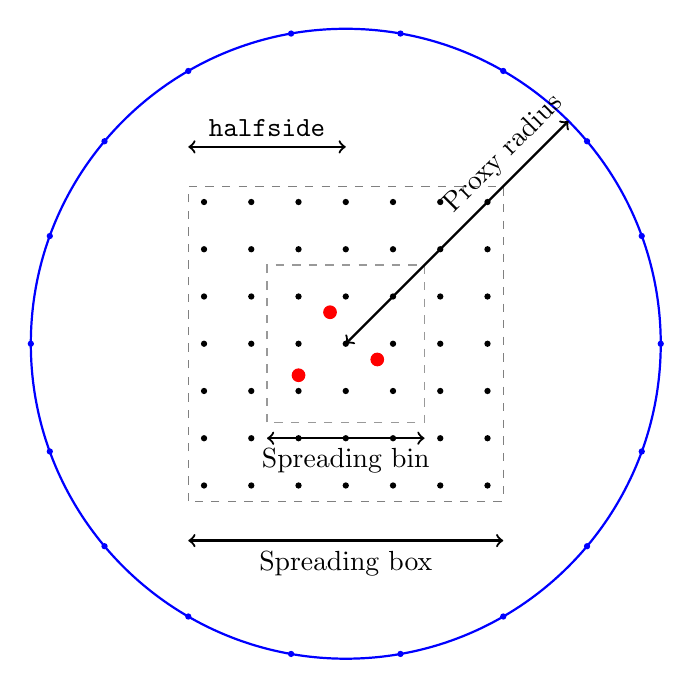
\begin{tikzpicture}[scale=2]
  % bounding square (spreading box)
  \draw[black!50, dashed] (-1,-1) rectangle (1,1);
  % inner box corresponding to halfside (from -0.5 to 0.5)
  \draw[black!40, dashed] (-0.5,-0.5) rectangle (0.5,0.5);

  % width arrow labeled 2 x halfside
  \draw[<->, thick] (-1,-1.25) -- (1,-1.25) node[midway, below] {Spreading box};
  \draw[<->, thick] (-1,1.25) -- (0,1.25) node[midway, above] {\halfside};

  \draw[<->, thick] (-0.5,-0.6) -- (0.5,-0.6) node[midway, below] {Spreading bin};

  % grid points (3x3 inside the inner box at -0.3, 0, 0.3)
  % chosen so no grid point sits on the inner box boundary at \pm0.5
  \foreach \x in {-0.9, -0.6, -0.3, 0, 0.3, 0.6, 0.9} {
    \foreach \y in {-0.9, -0.6, -0.3, 0, 0.3, 0.6, 0.9} {
      \fill[black] (\x,\y) circle (0.02);
    }
  }

  % source points (clustered inside)
  \filldraw[red] (-0.3,-0.2) circle (0.04); % node[black, right=2pt] {Source $x_j$};
  \filldraw[red] (-0.1,0.2) circle (0.04);
  \filldraw[red] (0.2,-0.1) circle (0.04);

  % proxy ring
  \draw[blue, thick] (0,0) circle (2);
  \foreach \t in {0,20,...,340} {
    \fill[blue] ( {2*cos(\t)}, {2*sin(\t)} ) circle (0.02);
  }

  % radius arrow from center to point on proxy ring at 45 degrees
  \draw[<->, thick] (0,0) -- ({2*cos(45)},{2*sin(45)}) node[midway, above right, rotate=45] {Proxy radius};


  % legend
%   \node[anchor=west] at (1.1,1.2) {\footnotesize Regular grid points};
%   \draw[black] (1.05,1.18) circle (0.02);
%   \node[anchor=west] at (1.1,1.0) {\footnotesize Proxy points};
%   \draw[blue, thick] (1.02,0.98) circle (0.02);
%   \node[anchor=west] at (1.1,0.8) {\footnotesize Source points};
%   \fill[red] (1.05,0.78) circle (0.04);
\end{tikzpicture}
\caption{Schematic of the spreading geometry in 2D: sources (red), the
regular discretization (black dots), and a proxy ring (blue).}
\end{figure}

\subsection{Computing the spreading box size}
The spreading box size is computed by \texttt{spread\_halfside()}. This is meant to approximately control the number of source points in a particular spreading box.

\subsection{Computing the regular grid spacing}
This is performed in \texttt{dx\_nproxy()}.
We want to find parameters \texttt{dx} and \texttt{nproxy}. \texttt{dx} is the grid spacing of the regular discretization of the spreading box, which starts at $-\halfside + \frac{\texttt{dx}}{2}$ and ends at $\halfside - \frac{\texttt{dx}}{2}$. \texttt{nproxy} is the number of proxy points placed on a proxy ring (or sphere) outside the spreading box.

Notes on the geometry used:
\begin{itemize}
    \item We put source points in a bin with sidelength $\texttt{c\_bwidth}  \times \halfside$.
    \item We place a proxy ring of radius $\sqrt{\texttt{d}} \times \halfside \times \texttt{crad}$ where \texttt{d} is the dimension (2 or 3) and \texttt{crad} is a constant (default 2.0).
    \item If we consider breaking the spreading box into \texttt{nspread} cells, the grid points are placed at the center of each cell, so $\texttt{dx} = \frac{2 \times \halfside}{\texttt{nspread}}$.
\end{itemize}


Notes on the algorithm used to compute \texttt{dx} and \texttt{nproxy}:
\begin{itemize}
  \item Generate random sources in the spreading bin with side length $\halfside$. Generate target points on a ring/sphere of radius $1.1 \times$ the proxy radius.
  \item Increase \texttt{nspread} and \texttt{nproxy} until the error tolerance is met.
  \item Decrease \texttt{nspread} until the error tolerance is no longer met.
  \item Spreading bin is $\texttt{dx} \times \texttt{nbinpts} = \texttt{dx} \times \lfloor \texttt{nspread}/2 \rfloor$.
  % \item Re-generate random source points inside a spreading bin of size $\texttt{dx} \times \lfloor \texttt{nspread}/2 \rfloor$, which may be slightly larger than the original spreading bin. Increase \texttt{nproxy} until the error tolerance is met.
\end{itemize}


\subsection{Constructing the regular grid}
This is performed in \texttt{get\_grid()}, which calls \texttt{spread\_halfside()} and \texttt{dx\_nproxy()}. Here are the basic steps:
\begin{itemize}
    \item Compute \texttt{halfside} using \texttt{spread\_halfside()}.
    \item Compute \texttt{dx}, \texttt{nspread}, and \texttt{nproxy} using \texttt{dx\_nproxy()}.
    \item Construct a bounding rectangle around the source points, which, along with the side length of the spreading bin, determines \texttt{ngrid}, the number of regular grid points in each dimension.
    \item Add a padding of grid points on each side so that the spreading bins fit properly into the corners of the bounding rectangle. $\texttt{pad} = \lceil (\texttt{nspread} - \texttt{nbinpts}) / 2 \rceil$.
    \item Start the regular grid points a bit below the bottom corner of the bounding rectangle. See \cref{fig:padding} for an illustration of this padding.
\end{itemize}

\begin{figure}
\centering
\begin{subfigure}{0.48\textwidth}
  \centering
  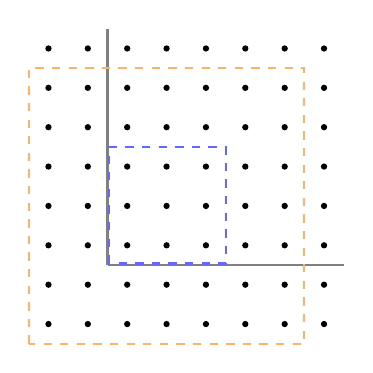
\begin{tikzpicture}[scale=2]
  % bounding rectangle
  % vertical line from (-1,-1) to (-1,1)
  \draw[black!50, thick] (-1,-1) -- (-1,0.5);
  \draw[black!50, thick] (-1,-1) -- (0.5,-1);
  % inner box corresponding to halfside (from -0.5 to 0.5)
  \draw[blue!60, dashed, thick] (-0.99,-0.99) rectangle (-0.25,-0.25);
  \draw[orange!60, dashed, thick] (-1.5, -1.5) rectangle (0.25,0.25);

  \foreach \x in {-1.375, -1.125, -0.875, -0.625, -0.375, -0.125, 0.125, 0.375} {
    \foreach \y in {-1.375, -1.125, -0.875, -0.625, -0.375, -0.125, 0.125, 0.375} {
      \fill[black] (\x,\y) circle (0.02);
    }
  }
\end{tikzpicture}
\caption{$\texttt{nbinpts}=3$, $\texttt{nspread}=7$}
\end{subfigure}
\begin{subfigure}{0.48\textwidth}
  \centering
  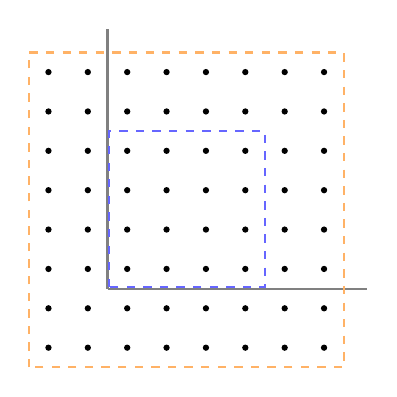
\begin{tikzpicture}[scale=2]
  % bounding rectangle
  % vertical line from (-1,-1) to (-1,1)
  \draw[black!50, thick] (-1,-1) -- (-1,0.65);
  \draw[black!50, thick] (-1,-1) -- (0.65,-1);
  % inner box corresponding to halfside (from -0.5 to 0.5)
  \draw[blue!60, dashed, thick] (-0.99,-0.99) rectangle (0,0);
  \draw[orange!60, dashed, thick] (-1.5, -1.5) rectangle (0.5,0.5);

  \foreach \x in {-1.375, -1.125, -0.875, -0.625, -0.375, -0.125, 0.125, 0.375} {
    \foreach \y in {-1.375, -1.125, -0.875, -0.625, -0.375, -0.125, 0.125, 0.375} {
      \fill[black] (\x,\y) circle (0.02);
    }
  }
\end{tikzpicture}
\caption{$\texttt{nbinpts}=4$, $\texttt{nspread}=8$}
\end{subfigure}
\caption{Schematic of the padding of the regular grid around the source points. 
The black lines form the bottom left corner of the bounding rectangle, the blue dashed line is the first spreading bin, and the orange dashed line is its associated spreading box. 
The regular grid points (black dots) start slightly below the bounding rectangle. 
There are $ \texttt{pad} = \lceil (\texttt{nspread} - \texttt{nbinpts}) / 2 \rceil$ extra grid points hanging below and to the left of the bounding rectangle to ensure proper padding for spreading.}
\label{fig:padding}
\end{figure}


\end{document}